\documentclass[twocolumn, a4paper]{UECIEresume}

\usepackage[dvipdfmx]{graphicx}
\usepackage{graphicx}
\usepackage{amsmath}
\usepackage{txfonts}

\title{レスキュー犬の一人称動画を用いた動作分類}
\date{平成 30 年 9 月 27 日}
\affiliation{総合情報学科 メディア情報学コース}
\supervisor{柳井啓二 教授}
\studentid{1730010}
\author{荒木勇人}
%\headtitle{平成 yy 年度 総合情報学科 卒業論文中間発表}
%\headtitle{平成 yy 年度 総合情報学科 卒業論文発表}
\headtitle{平成 30 年度 総合情報学科 修士論文中間発表}
%\headtitle{平成 yy 年度 総合情報学科 修士論文発表}

\begin{document}
\maketitle

\section{はじめに}
被災地での救助活動を行う際に,人間だけでは不十分な場合がある.そこで,人間に代わって探査を行うのが訓練されたレスキュー犬(災害救助犬)である.レスキュー犬は,がれきの隙間などの狭い空間,倒壊した建物など踏破困難な環境でも探査可能であり,また人間より発達した嗅覚を頼りにした救助活動が可能である.しかし,彼らは人間に向けた言語を持たないため,人間はレスキュー犬の行動から彼らが収集した情報を理解しなくてはならない.現状では,災害救助犬を指揮するハンドラーと呼ばれる人間がレスキュー犬の行動を手動でマーキングしており,その情報を消防などの指揮命令者に口頭伝達している.この問題点として,トリアージ(緊急度に従った手当の優先順位付け)のための周辺環境情報や,要救助者の情報量の不足や客観性の不足があげられる.

レスキュー犬の行動をモニタリングするために,装着型計測・記録装置が開発された~\cite{dog01}.これは,各種センサを用いた計測データを記録し,リアルタイムに映像などのデータを無線配信している.本研究では,これらのデータを用いてレスキュー犬の行動をリアルタイムに分類すること目的とする.深層学習を用いた動画識別にある既存手法を予備実験として行った.動画識別のための新規性としては,映像だけでなく音声などのデータを使ったマルチモーダルな画像分類という点があげられる.
レスキュー犬が今何をしているのかが明示的に判明することで,トリアージに必要な情報が整理され,災害救助活動の効率化が期待される.

\section{関連研究}
一人称視点動画の分類に関する研究


\section{予備実験}
データセットに犬の一人称視点動画DogCentric Activity Dataset~\cite{yumi2014first}を用い,これを分類する予備実験を行った.動画ひとつにつき各フレームの平均を取り,
画像として分類した.DogCentric Activity Dataset のみでの学習~\ref{model}と,VGG16\cite{vgg16}を用いたPre-trained model~\ref{vgg16model}のfine-tuningと二通り行った.
\begin{figure}[b]
 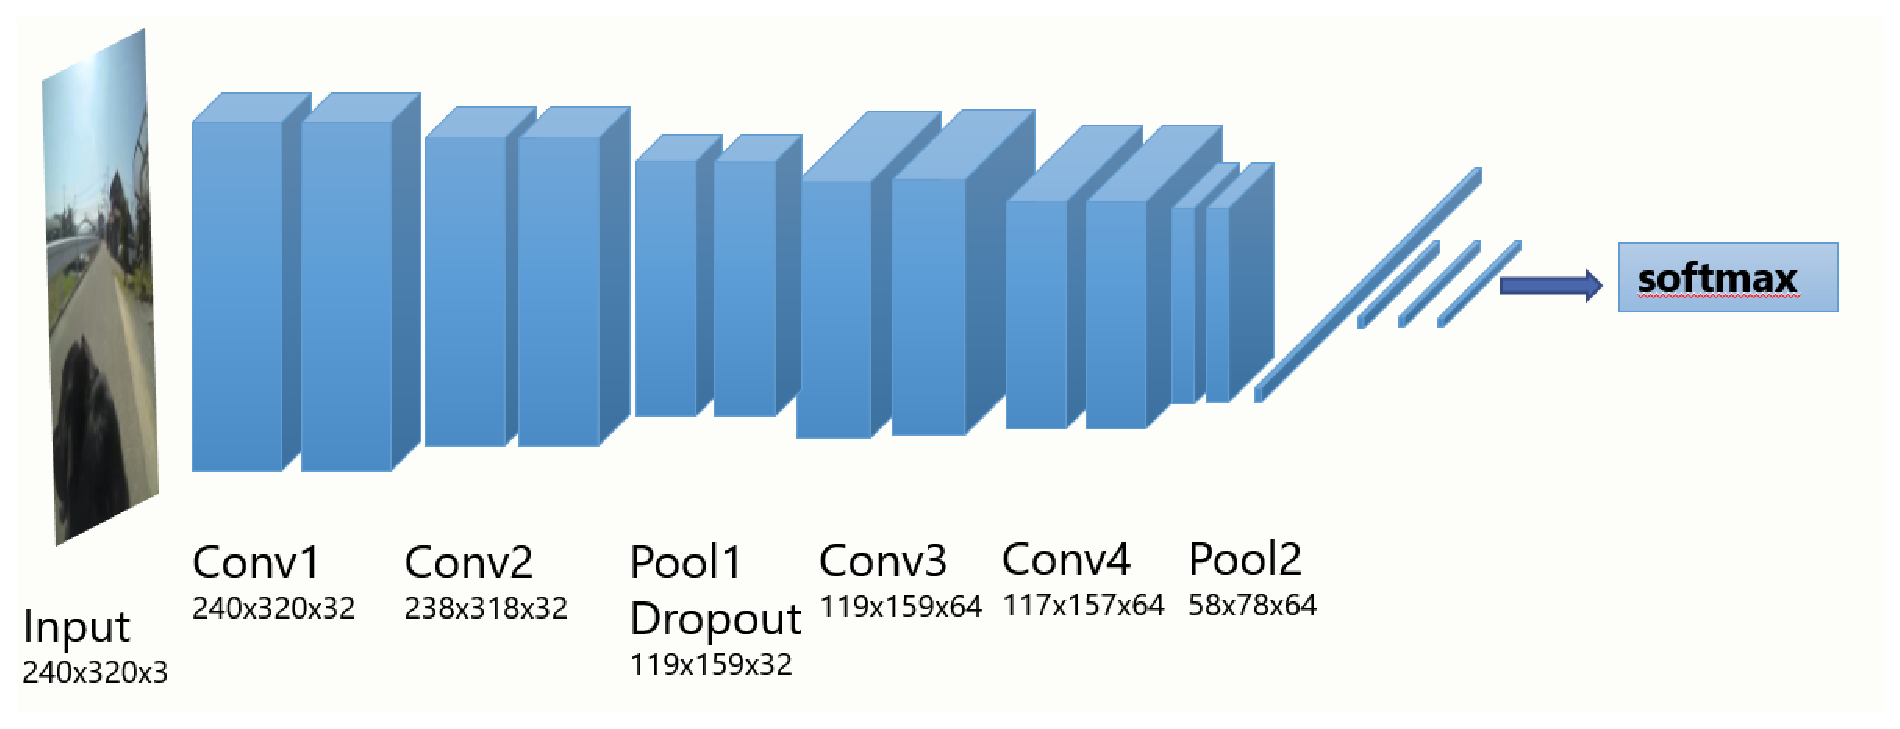
\includegraphics[width=10cm]{./Img/usemodel.eps}
 \caption{利用したモデル}
 \label{model}
\end{figure}
\begin{figure}[b]
 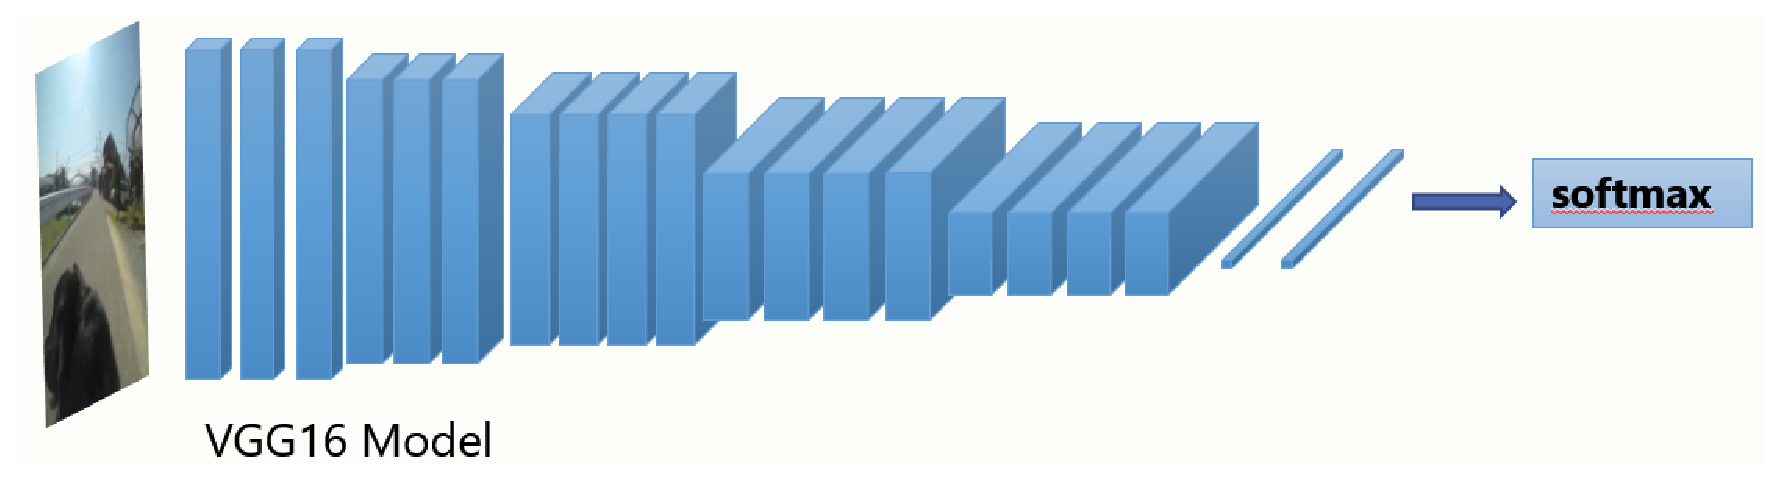
\includegraphics[width=10cm]{./Img/vgg16model.eps}
 \caption{VGG16モデル}
 \label{vgg16model}
\end{figure}

\section{まとめ,今後の課題}
\begin{itemize}
  \item{test}
  \item{test2}
\end{itemize}

\begin{footnotesize}
%{\small
\bibliographystyle{junsrt}
\bibliography{ref}
%}
\end{footnotesize}
\end{document}
